
\documentclass[12pt]{article}

%%%%%%%%%%%%%%%%%%%%%%%%%%%%%%%%%%%%%%%%%%%%%%%%%%%%%%%%%%%%%%%%%%%%%%%%%%%%%%%
% PACKAGE INCLUDING
%%%%%%%%%%%%%%%%%%%%%%%%%%%%%%%%%%%%%%%%%%%%%%%%%%%%%%%%%%%%%%%%%%%%%%%%%%%%%%%
\usepackage{amsmath}
\usepackage{graphicx}
\usepackage{hyperref}
\usepackage[utf8]{inputenc}
\usepackage[T5]{fontenc}
\usepackage{fancyhdr}
\usepackage{geometry}

\usepackage{csquotes}
\usepackage{listings}
\usepackage{enumitem}
\usepackage{subfiles}
\usepackage{tcolorbox}
\usepackage{colortbl}
\usepackage{float}
\usepackage{circuitikz}
\usepackage{tikz}
\usepackage{bm}
%%%%%%%%%%%%%%%%%%%%%%%%%%%%%%%%%%%%%%%%%%%%%%%%%%%%%%%%%%%%%%%%%%%%%%%%%%%%%%%
% FORMATTING
%%%%%%%%%%%%%%%%%%%%%%%%%%%%%%%%%%%%%%%%%%%%%%%%%%%%%%%%%%%%%%%%%%%%%%%%%%%%%%%
\geometry{
    a4paper,
    total={170mm,250mm},
    left=20mm,
    top=30mm,
 }
\hypersetup{
    colorlinks=true,
    linkcolor=blue,
    filecolor=magenta,      
    urlcolor=blue,
    citecolor=blue
}

\pagestyle{fancy}
\fancyhf{}
\rhead{19120729}
\lhead{Bùi Ngọc Thảo Vy}
\rfoot{Trang \thepage}\setlength{\parindent}{0pt}
\setlength{\parskip}{0.3em}
\setlength{\headheight}{15pt}
\graphicspath{ {./images/} }

\setcounter{secnumdepth}{4}
\setcounter{tocdepth}{4}

\usetikzlibrary{matrix,calc}

%%%%%%%%%%%%%%%%%%%%%%%%%%%%%%%%%%%%%%%%%%%%%%%%%%%%%%%%%%%%%%%%%%%%%%%%%%%%%%%
% DEFINE NEW COMMAND
%%%%%%%%%%%%%%%%%%%%%%%%%%%%%%%%%%%%%%%%%%%%%%%%%%%%%%%%%%%%%%%%%%%%%%%%%%%%%%%
\newcommand{\SubItem}[1]{
    {\setlength\itemindent{15pt} \item[-] #1}
}

%%%%%%%%%%%%%%%%%%%%%%%%%%%%%%%%%%%%%%%%%%%%%%%%%%%%%%%%%%%%%%%%%%%%%%%%%%%%%%%
% DOCUMENT
%%%%%%%%%%%%%%%%%%%%%%%%%%%%%%%%%%%%%%%%%%%%%%%%%%%%%%%%%%%%%%%%%%%%%%%%%%%%%%%
\title{Kiểm tra kết thúc học phần môn Toán tổ hợp}

\author{LỚP 19CTT4}

\date{2021–07–05}


\begin{document}
\begin{sloppypar}

\begin{titlepage}
    
    \newcommand{\HRule}{\rule{\linewidth}{0.5mm}} % Defines a new command for the horizontal lines, change thickness here
    
    \center % Center everything on the page
    \vspace*{\fill}
     
    \textsc{\LARGE Đại học Khoa học Tự nhiên}\\[0.2cm]
    \textsc{\large Đại học Quốc gia TP. HCM }\\[1.5cm] 
    \textsc{\Large KHOA CÔNG NGHỆ THÔNG TIN}\\[0.2cm] 
    \textsc{\large LỚP 19CTT4 }\\[0.5cm]
    \HRule \\[0.4cm]
    { \huge \bfseries Kiểm tra kết thúc học phần môn\break 
    Thực hành Toán tổ hợp}\\[0.4cm] % Title of your document
    \HRule \\[1.5cm]
    \LARGE \textbf {Họ và tên: Bùi Ngọc Thảo Vy \\}
    \LARGE \textbf {MSSV: 19120729 \\}
    
    \begin{minipage}{1\textwidth}
    \begin{center}
        \LARGE Ngày 05/07/2021
    \end{center}
    \end{minipage}\\[2cm]
    \vspace*{\fill} % Fill the rest of the page with whitespace
    \end{titlepage}


    % MỤC LỤC
    \renewcommand*\contentsname{\begin{center} \LARGE Mục lục \end{center}}
    \tableofcontents
    \pagebreak
\section{Bài 1}
\subsection{Câu A: Lên cầu thang}

\begin{tcolorbox}
    \textbf{Đề bài:} Một cầu thang có \(n\) bậc, mỗi lần bước có thể bước lên 1 bậc hay 2 bậc. Có bao nhiêu cách đi hết cầu thang này? (đây chính là dãy Fibonaxi)
\end{tcolorbox}

- Gọi \(a_{n}\) là số cách bước lên cầu thang có \(n\) bậc. \\
- Do một lần có thể bước lên 1 hoặc 2 bậc nên ta có 2 cách để bước lên bậc thang thứ \(n\):

\begin{itemize}
    \item Từ bậc \(n - 1\)
    \item Từ bậc \(n - 2\)
\end{itemize}

- Với mỗi cách, ta lần lượt có \(a_{n-1}\) và \(a_{n - 2}\) cách. \\
\begin{center}
    {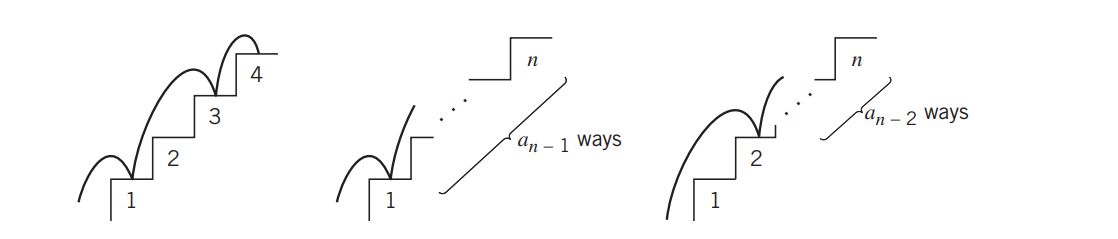
\includegraphics[width=16cm]{ex1a.png}}
\end{center}
- Teho nguyên lý cộng, ta có:

\begin{equation*}
    a_{n} = a_{n-1} + a_{n-2}
\end{equation*}

- Để bước lên bậc thang thứ 1, ta có 1 cách \(\Rightarrow a_{1} = 1\) \\
- Để bước lên bậc thang thứ 2, ta có 2 cách \(\Rightarrow a_{2} = 2\) \\
- Mà, ta lại có \(a_{2} = a_{0} + a_{1} \Leftrightarrow a_{0} = a_{2} - a_{1} = 2 - 1 = 1\). Từ đó suy ra:


    \[
    \begin{cases}
        a_{n} & = a_{n-1} + a_{n-2} \\             
        a_{0} & = a_{1} = 1; a_{2} = 2   
    \end{cases}
    \]

- Sử dụng Maple để giải hệ thức đệ quy, ta được:

\begin{verbatim}
    f := rsolve({a(0) = 1, a(1) = 1, a(n) = a(n-1) + a(n-2)}, a(n)): simplify(f)
\end{verbatim}

\begin{equation*}
    a_{n} = \left(\frac{1}{2} - \frac{\sqrt{5}}{10}\right)\left(\frac{-\sqrt{5}}{2} + \frac{1}{2}\right)^{n} + \left(\frac{1}{2} + \frac{\sqrt{5}}{10}\right)\left(\frac{\sqrt{5}}{2} + \frac{1}{2}\right)^{n}
\end{equation*}

\subsection{Câu B: Chia mặt phẳng}
\begin{tcolorbox}
    \textbf{Đề bài:} Tìm số miền tối đa có thể có khi chia mặt phẳng bởi \(n\) đường thẳng.
\end{tcolorbox}

\begin{center}
    {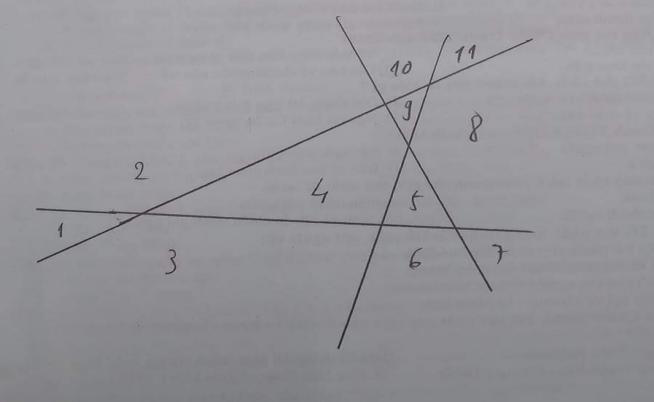
\includegraphics[width=8cm]{1b.png}}
\end{center}

- Gọi \(a_{n}\) là số mặt phẳng tối đa có thể có khi chia mặt phẳng bởi \(n\) đường thẳng. \\
- Đầu tiên, chúng ta khảo sát số miền tối đa có thể có đối với các giá trị \(n\) đường thẳng ban đầu như sau:

\begin{itemize}
    \item Với 0 đường đẳng (\(n = 0\)), ta thu được 1 mặt phẳng \(\Rightarrow a_{0} = 1\)
    \item Với 1 đường đẳng (\(n = 1\)), ta thu được 2 mặt phẳng \(\Rightarrow a_{1} = 2\)
    \item Với 2 đường thằng (\(n = 2\)), ta thu được 4 mặt phẳng \(\Rightarrow a_{2} = 4\)
    \item Với 3 đường thẳng (\(n = 3\)), ta thu được 7 mặt phẳng \(\Rightarrow a_{3} = 7\)
\end{itemize}

\begin{center}
    {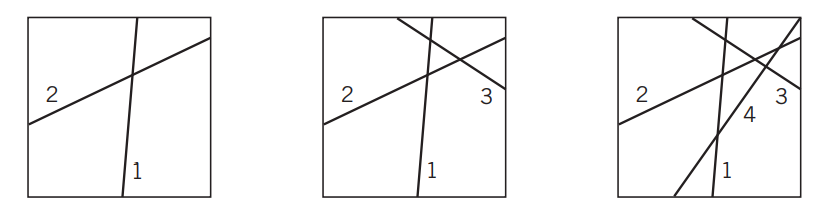
\includegraphics[width=16cm]{ex1b.png}}
\end{center}

- Như vậy, ta được dãy như sau:

\begin{equation*}
    a_{n} = a_{n - 1} + a_{n}
\end{equation*}

- Từ đó suy ra:

\[
    \begin{cases}
        a_{n} & = a_{n - 1} + n \\             
        a_{0} & = 1; a_{1} = 2   
    \end{cases}
    \]

- Sử dụng Maple để giải hệ thức đệ quy, ta được:

\begin{verbatim}
    f := rsolve({a(0) = 1, a(1) = 2, a(n) = a(n-1) + n}, a(n)): simplify(f)
\end{verbatim}

\begin{equation*}
    a_{n} = \frac{1}{2}n^{2} + \frac{1}{2}n + 1
\end{equation*}

\subsection{Câu C: Tháp Hà Nội}
\begin{tcolorbox}
    \textbf{Đề bài:} Có 3 cột 1,2 và 3. Có \(n\) đĩa nằm ở cột 1 được sắp xếp theo bán kính nhỏ dần từ dưới lên trên. Tìm số lần tối thiểu để chuyển tất cả n đĩa này sang cột khác sao cho thỏa mãn quy tắc:  đĩa có bán kính nhỏ hơn luôn nằm ở trên.
\end{tcolorbox}

\begin{center}
    {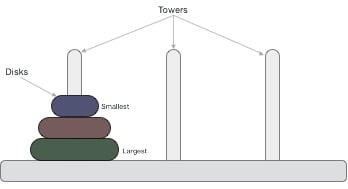
\includegraphics[width=8cm]{toh.png}}
\end{center}

\section{Bài 2}

\subsection{Câu A: Lãi suất ngân hàng}
\begin{tcolorbox}
    \textbf{Đề bài:} Ngân hàng Fe-credit (thật ra là cho vay nặng lãi) trả lãi suất 4\% mỗi năm từ số tiền tiết kiệm (lãi kép). Tìm quan hệ đệ quy của số tiền rút ra sau n năm trong 2 trường hợp sau đây: \\ \\
    I)  Gửi vào 1000\$ và lấy ra sau \(n\) năm. \\
    II) Gửi vào 100\$ mỗi cuối năm.
\end{tcolorbox}

\subsection{Câu B}
\begin{tcolorbox}
    \textbf{Đề bài:} Có bao nhiêu cách tổ hợp \(n\) \$ theo các tờ tiền có mệnh giá là 1\$, 5\$ và 10\$. Có quan tâm đến thứ tự của các mệnh giá.
\end{tcolorbox}

\subsection{Câu C: Dãy con bị cấm}
\begin{tcolorbox}
    \textbf{Đề bài:} Tìm quan hệ đệ quy cho \(a_{n}\), số chuỗi tam phân có độ dài \(n\) mà không xuất hiện chuỗi con “012”.
\end{tcolorbox}

\section{Bài 3}
\subparagraph {Sử dụng maple để giải quyết 2 bài toán sau đây:}

\subsection{Câu A}
\begin{tcolorbox}
    \textbf{Đề bài:} Tính tổng \(1.2.3.4 + 2.3.4.5 + ....... + n.(n+1).(n+2).(n+3)\)
\end{tcolorbox}

\subsection{Câu B}
\begin{tcolorbox}
    \textbf{Đề bài:} Tìm số các phân hoạch của số nguyên 10 dựa vào hàm sinh.
\end{tcolorbox}

\section{Bài 4}
\begin{tcolorbox}
    \textbf{Đề bài:}  Gọi \(A_{n}\) là số cách sắp xếp các số nguyên từ 1 đến \(n\) sau cho số nguyên \(i\) không nằm liền sau số nguyên \(i+1\) 
    (với \(i=1,...,n-1\)). Và Dn là số các xáo trộn của tập hợp các số nguyên từ 1 đến \(n\). Chứng minh rằng \(A_{n}= D_{n} + D_{n-1}\)
\end{tcolorbox}

\section{Bài 5}
\begin{tcolorbox}
    \textbf{Đề bài:} Hàm euler \(p(n)=\) số các số nguyên từ \(1\) đến \(n\) và nguyên tố cùng nhau với \(n\). Sử dụng nguyên lý bù trừ để tính \(p(n)\) dựa vào phân tích của \(n\) ra thừa số nguyên tố. Áp dụng: tính \(p(100)\).
\end{tcolorbox}

\section{Bài 6: Đa thức sắc tố đồ thị(chromatic polynomial)}
\begin{tcolorbox}
    \textbf{Đề bài:} Cho đồ thị G đơn, vô hướng như hình bên dưới.  Sử dụng nguyên lý bù trừ để tính số cách tô màu 4 đỉnh của đồ thị với  \(n\) màu cho trước sao cho các đỉnh kề nhau được tô bởi các màu khác nhau. ( đỉnh là \(x_{i}\), cạnh là \(e_{i}\) )
\end{tcolorbox}

\begin{center}
    {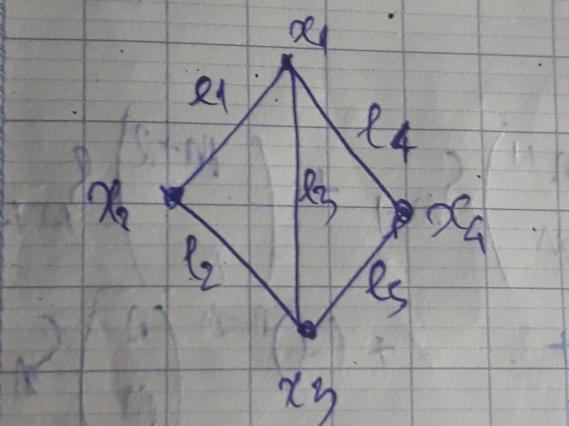
\includegraphics[width=8cm]{6.png}}
\end{center}

\section{Bài 7}
\begin{tcolorbox}
    \textbf{Đề bài:} Chứng minh rằng số cây khung của đồ thị đầy đủ \(K_{n}\) là \(n^{n-2}\).
    (với \(n > 1\)).
\end{tcolorbox}

\section{Bài 8: Bài toán đường đi tránh vũng nước}
\begin{tcolorbox}
    \textbf{Đề bài:} Tìm thuật toán để giải quyết bài toán sau đây: Xét góc phần tư thứ I của hệ trục tọa độ \(Oxy\) với các lưới nguyên (giống như giấy tập có ô), có một vũng nước S ( là một tập hợp các điểm nguyên nằm trong I).
    (với \(n > 1\)).
\end{tcolorbox}

\begin{center}
    {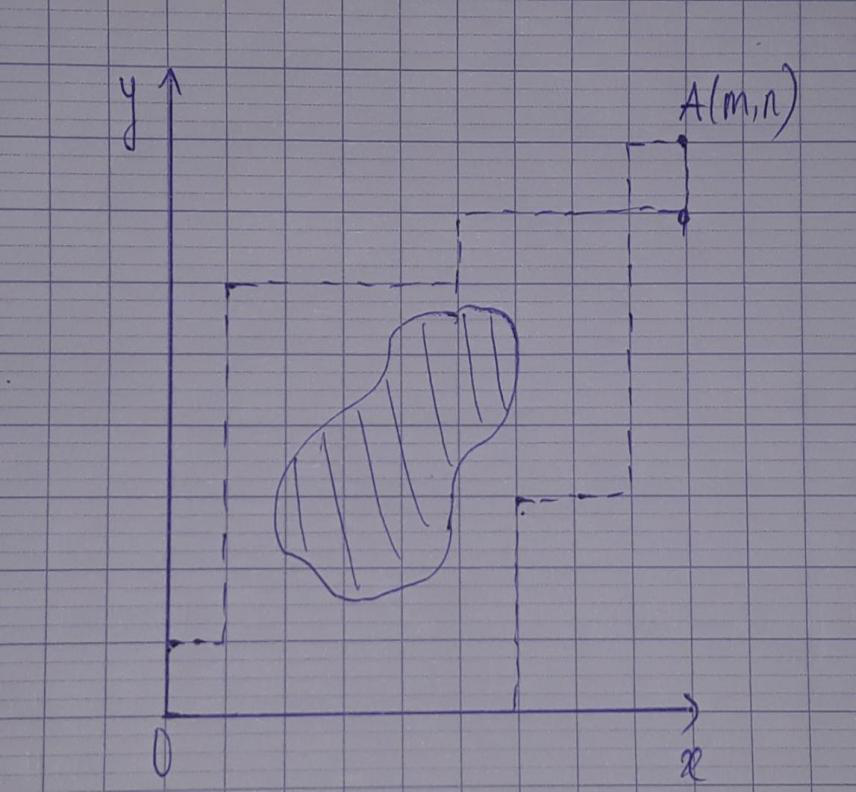
\includegraphics[width=8cm]{7.png}}
\end{center}

\subsection{Câu A}
\begin{tcolorbox}
    \textbf{Đề bài:} A)Tìm số đường đi từ O đến A tránh vũng nước S biết mỗi lần đi, chỉ được lên trên 1 đơn vị hoặc qua phải 1 đơn vị.
\end{tcolorbox}
\subsection{Câu B}
\begin{tcolorbox}
    \textbf{Đề bài:} B)Có nhận xét gì về số đường đi như vậy nếu vũng nước S không tồn tại.
\end{tcolorbox}

\section{Bài 9}
\begin{tcolorbox}
    \textbf{Đề bài:} Xét bài toán trên, tính số đường đi từ O đến A(n,n) và S là nửa mặt phẳng phía trên OA không kể bờ.
\end{tcolorbox}

\section{Bài 10}
\begin{tcolorbox}
    \textbf{Đề bài:} Cho một hình chữ nhật \(mxn\). C là một bàn cờ nằm trong HCN này và \(C’\) là phần còn lại của \(C\) trong HCN đó.
    Chứng minh rằng \(R(x,C’)=x^{n} .R(1/x,C)\). Gợi ý: bt 15/351 quyển Applied Combinatorics.
\end{tcolorbox}

\section{Bài 11: Định lý thặng dư Trung Hoa}
\begin{tcolorbox}
    \textbf{Đề bài:} Trước khi tiến hành thi học kì, toàn bộ sinh viên đh khtn bắt buộc phải được lấy mẫu tầm soát covid. Để biết chính xác có bao nhiêu sinh viên tham gia, chúng ta làm như sau (nhanh hơn và chính xác hơn việc đếm rất nhiều).
    Đầu tiên cho sinh viên tập trung trong khuôn viên trường là hình vuông cạnh 100m, để đảm bảo an toàn nên các bạn sinh viên đứng cách đều nhau. Lấy một ô đơn vị làm mẫu có kích thước 20m x 20m, ta dự đoán được trong đó có khoảng từ 490 đến 500 sinh viên. Sau đó chúng ta sẽ cho tất cả sinh viên xếp thành các hàng 5,7 và 11. Trong mỗi lần xếp như vậy, số sinh viên dư ra lần lượt là 0,4 và 3. Hãy tính chính xác số lượng sinh viên. (bởi vì dù chỉ 1 người chưa được tầm soát cũng rất nguy hiểm)
\end{tcolorbox}
\end{sloppypar}
\end{document}